% !TEX root = ../main.tex

\appendix

\section{Appendix}

\subsection{Sensitivity analysis}

\begin{figure}[H]
    \centering
    \makebox[\textwidth][c]{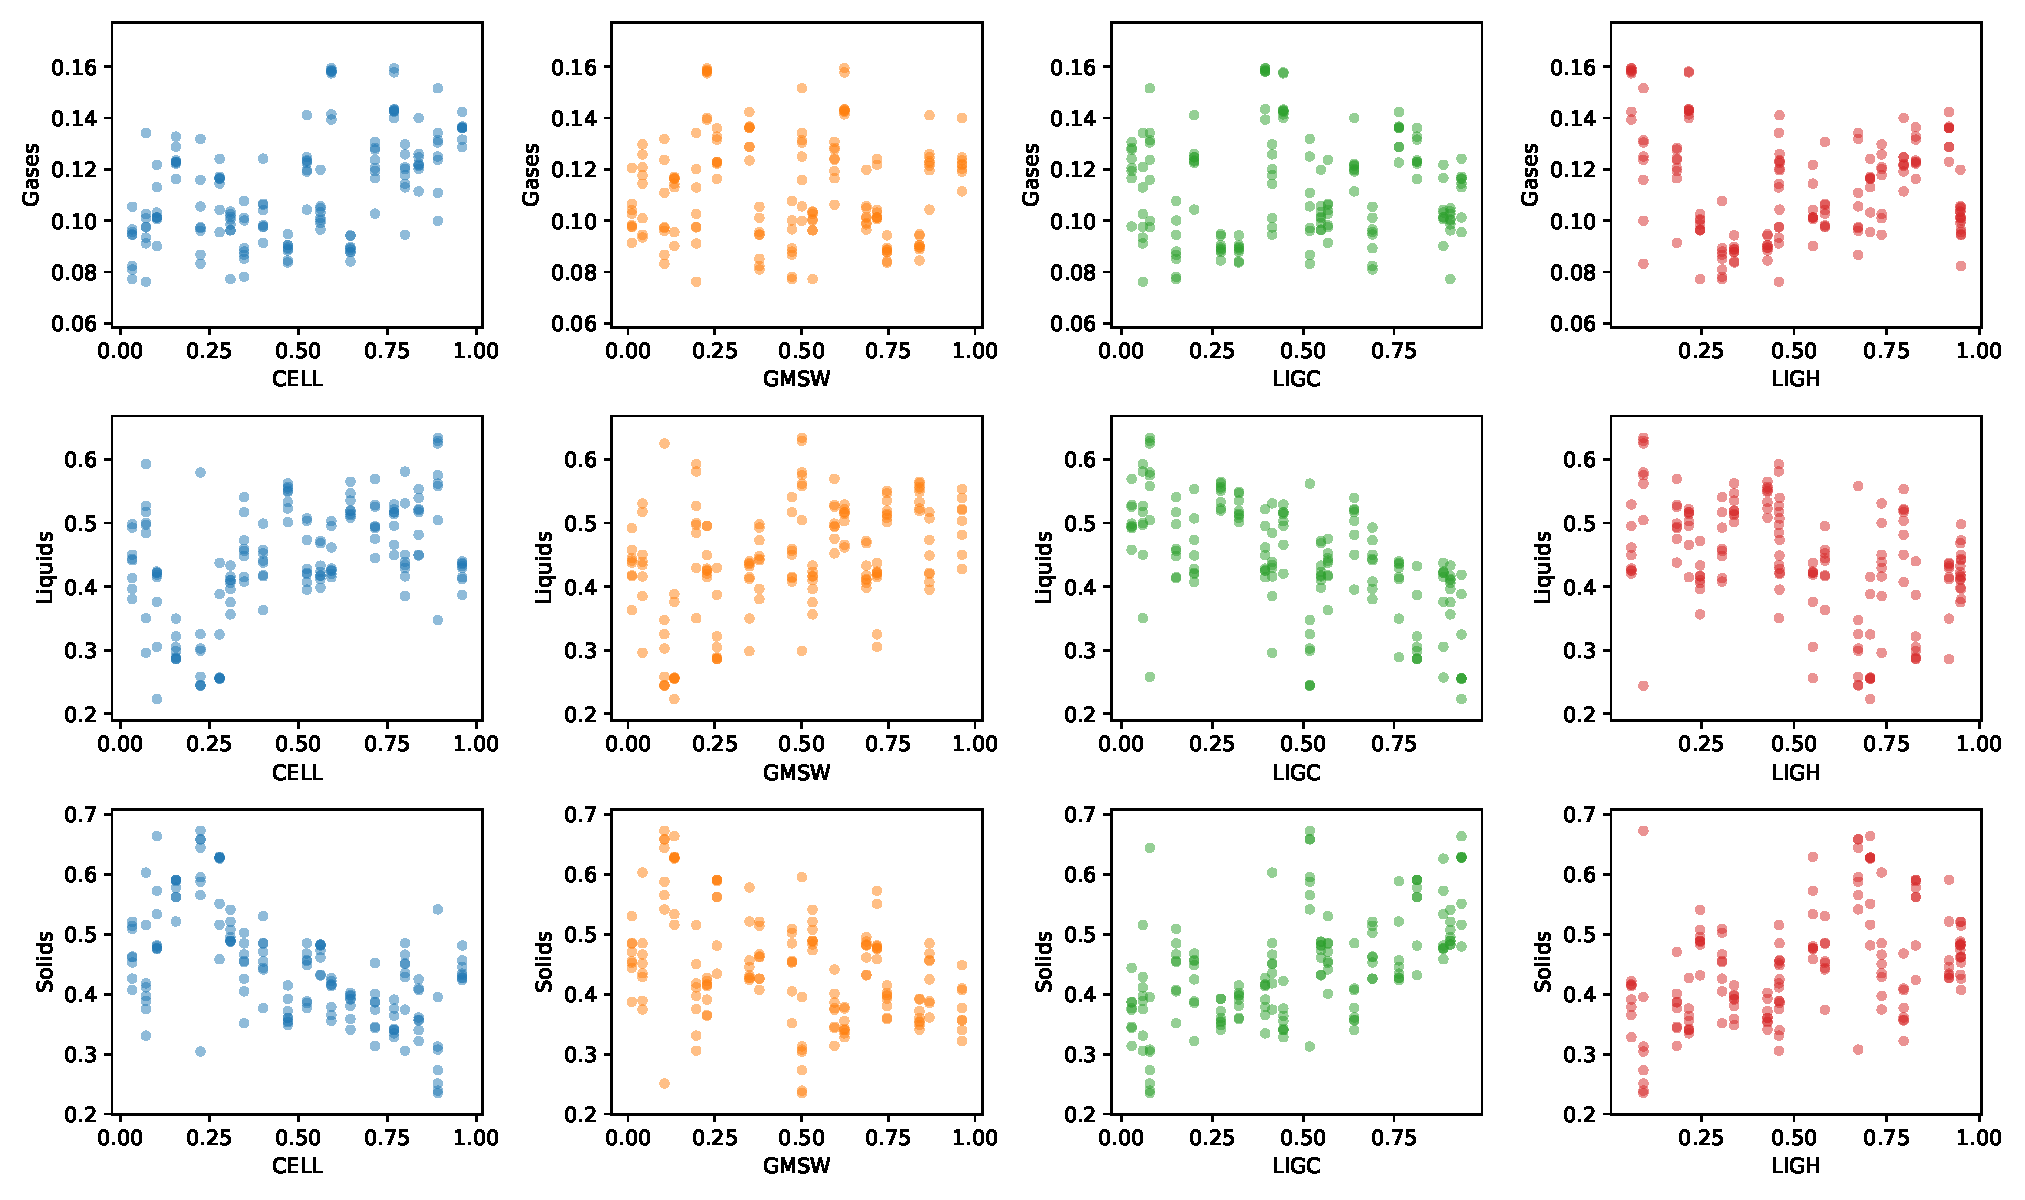
\includegraphics[width=1.3\textwidth]{figures/sa-scatter1-n10.pdf}}
    \caption{Batch reactor results for cellulose, hemicellulose (GMSW), carbon-rich lignin (LIGC), and hydrogen-rich lignin (LIGH) using 160 samples. Reaction time is 10 seconds at 773.15 K and 101,325 Pa.}
\end{figure}

\begin{figure}[H]
    \centering
    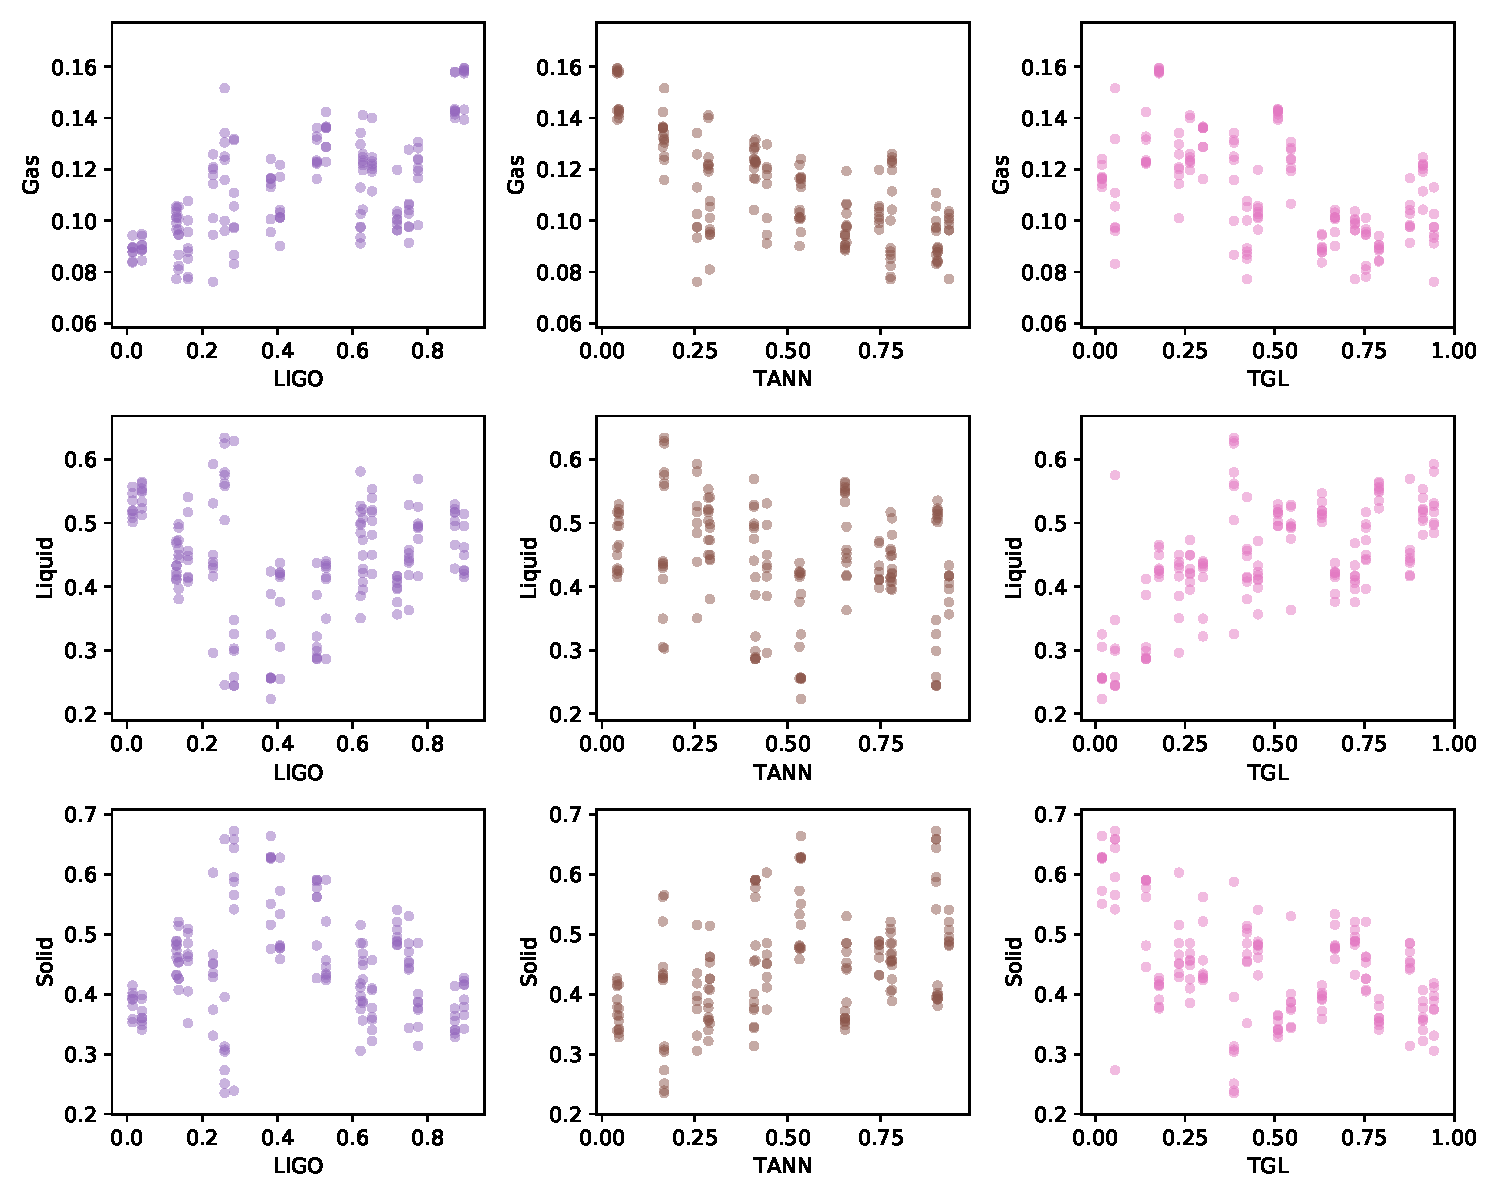
\includegraphics[width=\textwidth]{figures/sa-scatter2-n10.pdf}
    \caption{Batch reactor results for oxygen-rich lignin (LIGO), tannins (TANN), and triglycerides (TGL) using 160 samples. Reaction time is 10 seconds at 773.15 K and 101,325 Pa.}
\end{figure}

\begin{figure}[H]
    \centering
    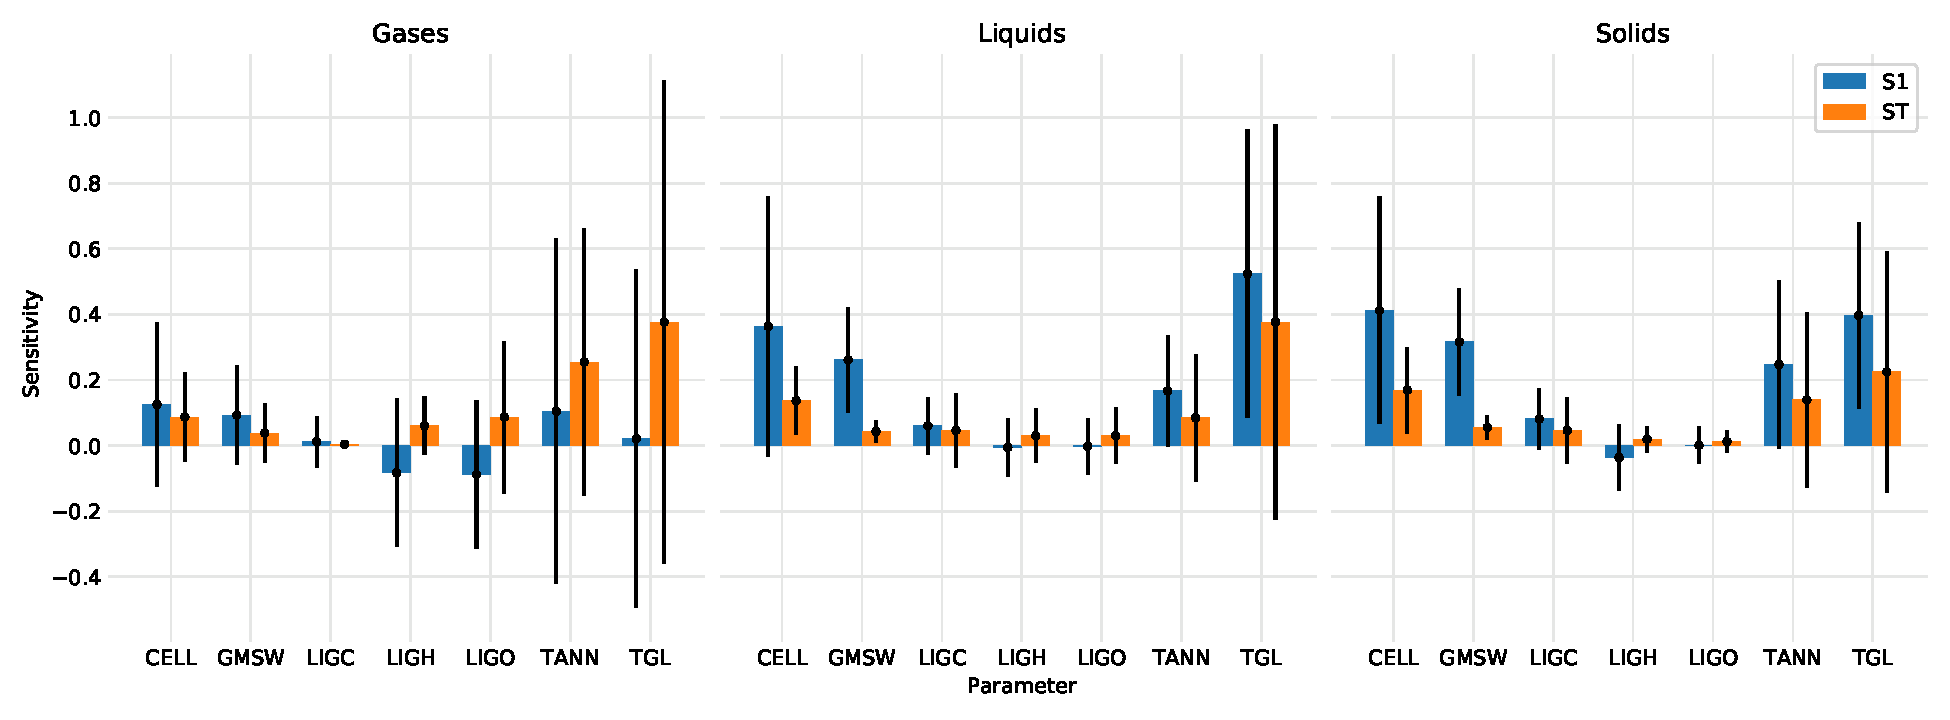
\includegraphics[width=\textwidth]{figures/sa-bar-n10.pdf}
    \caption{First-order (S1) and total-order (ST) Sobol indices for biomass composition with reactants grouped as gases, liquids, and solids using 160 samples.}
\end{figure}
